\chapter{Méthodes de représentation et d'analyse de l'architecture CxSOM}
\graphicspath{{03-Representation/}}
\minitoc

Dans le chapitre précédent, nous avons proposé l'algorithme CxSOM permettant de construire des architectures non-hiérarchiques de cartes auto-organisatrices.
Parallèlement à l'objectif d'une SOM, qui consiste à effectuer de la quantification vectorielle sur un espace d'entrée, l'objectif d'une architecture de SOM est de faire de la quantification vectorielle sur plusieurs espaces d'entrées et d'apprendre les relations entre ces entrées.
C'est ce qu'on appelle mémoire associative. Le but de cette thèse est d'analyser dans quelle mesure, et de quelle façon un tel apprentissage se déroule grâce au modèle CxSOM.

En utilisant une architecture sur ces entrées, on a deux objectifs. D'abord, on cherche à ce que chaque carte joue un rôle similaire à celui d'une carte de Kohonen classique, par rapport à son entrée externe.
Chaque carte prise séparément doit donc avoir appris une représentation de son espace d'entrée, en présentant une continuité entre les prototypes.
Ensuite, on souhaite aussi que le modèle liant les entrées soit appris par l'architecture. Cet aspect est nouveau:
nous introduirons des modes de représentation cherchant à définir l'existence d'un apprentissage du modèle, et comment le mesurer.

Ce chapitre a pour but d'étudier l'organisation d'une architecture simple, tout en indroduisant les méthodes et les représentations que nous utiliserons par la suite.
Nous présenterons la méthode expérimentale sur une architectures de deux cartes, et observerons son comportement grâce aux différents modes de représentations.
Nous introduirons également un indicateur caractérisant l'organisation d'une architecture, consruit à partir de l'information mutuelle.


\subsection{Représentations et indicateurs classique des cartes de Kohonen}

Les cartes de Kohonen sont particulièrement associées à une facilité de représentation et de visualisation. Leur nombre réduit de prototypes et leur aspect topologique permet d'en tracer une représentation visuelle interprétable.
La manière la plus couramment utilisée de représenter une carte de Kohonen est de tracer les poids de ses prototypes, disposés dans le graphe (ligne ou grille) qu'est la carte. En fonction des dimensions des entrées, cette représentation prennent plusieurs formes. Deux exemples courants de représentation sont les suivants: 
\begin{itemize}
\item Le graphe qu'est la carte de Kohonen est représenté dans l'espace de ses positions (la grille d'indices $(i,j)$, ou une ligne indexée par $i$. Sur chaque noeud est tracé le poids correspondant. C'est le cas sur l'exemple de gauche en figure~\ref{fig:representation} dans lequel les poids des prototypes, qui sont des imagettes, sont affichés en chaque point de la grille. Si la dimension d'un poids est trop grande pour être représentée graphiquement, il est également courant d'étiquetter chaque prototype et d'afficher ces étiquettes sur les noeuds de la carte, en tant que représentation.
\item Lorsque les données traitées sont des points deux ou trois dimensions, les poids des prototypes peuvent être directement tracés dans l'espace $\mathbb{R}^2$ ou $\mathbb{R}^3$. Ces poids sont alors reliés en fonction des positions des noeuds dans la carte, montrant ainsi la déformation de la carte dans l'espace d'entrée, c'est le cas sur l'exemple de droite en figure~\ref{fig:representation}.
\end{itemize}

\begin{figure}
\begin{minipage}{0.5\textwidth}
\centering
\includegraphics[width=0.5\textwidth]{digits.jpg}
\end{minipage}
\begin{minipage}{0.5\textwidth}
\centering
\includegraphics[width=0.5\textwidth]{points.png}
\end{minipage}
\label{fig:representation}
\caption{Représentations possible des poids d'une carte de Kohonen classiques, dans le cas d'entrées sous forme d'imagettes ou de points en deux dimensions.}
\end{figure}

\subsection{Limite de la représentation classique pour CxSOM}

Nous pouvons tracer les poids de chaque carte de l'architecture après apprentissage. On considère que les cartes ont atteint la fin de l'apprentissage lorsque les poids ne varient plus que peu.
La figure~\ref{fig:weights} présente le tracé des poids des deux cartes de l'exemple. Ce tracé permet de conclure que les cartes sont bien dépliées: les poids présentent une continité dans l'espace d'entrée.

On aimerait mieux comprendre les mécanismes impliqués dans l'apprentissage de ces cartes. Or, le choix du BMU dépend de plusieurs entrées et du processus de relaxation. La représentation des poids seuls ne permet pas de comprendre quels seront les BMUs de chaque carte pour une entrée donnée. 
Par ailleurs, représenter les cartes une à une laisse de coté leur connexion. Il est donc nécessaire de trouver un moyen de représenter l'architecture comme un tout. La représentation cherchera notamment à montrer comment l'architecture de cartes est capable d'apprendre les relations entre les entrées multimodales.

Enfin, la représentation visuelle d'une cartes d'une architecture est limitée par la dimension des entrées et la dimension des cartes. Dans l'exemple, les entrées et les cartes sont en une dimension, représenter leurs poids est donc réalisable; en plus grande dimension, il sera nécessaire d'utiliser une représentation telle que celle décrite en figure~\ref{fig:representation}. Le nombre de connexions contextuelles limitera alors également la lecture d'un tracé. Cette difficulté de représentation soulève la nécessité de définir des valeurs indicatrices du fonctionnement de la carte, calculables en grande dimension.

\begin{figure}
\centering
\includegraphics[width=0.9\textwidth]{weights_cercle1.pdf}
\label{fig:weights}
\caption{Représentation des valeurs des poids d'une carte au sein de CxSOM après apprentissage. La seule représentation de ces poids ne suffit pas à savoir comment la carte se comporte.}
\end{figure}

Ce chapitre questionne donc la façon de représenter une carte au sein d'une architecture. Nous présenterons en premier lieu un formalisme décrivant les cartes et leurs entrées multimodales associées. A partir de ce formalisme, nous proposerons plusieurs représentations et indicateurs permettant de comprendre et représenter ce que calcule une architecture CxSOM sur les données d'entrées. Nous utiliserons ces représentations et indicateurs dans les chapitres suivants. 

\section{Formalisme: variables aléatoires}

Nous introduisons dans cette section un formalisme traitant les éléments des cartes et les entrées en tant que variables aléatoires. Ce formalisme a l'avantage de à la fois clarifier les représentations, et de permettre le développement d'indicateurs statistiques sur les cartes.

\subsection{Représentation des entrées}

Les observations multimodales que l'on cherche à apprendre par l'architecture de cartes sont notées $(\inpx\m{i}, i = 1 \cdots n)$ où $n$ est le nombre de modalités considérées. On considère les $\inpx\m{i}$ comme des variables aléatoires, et le vecteur $\mathbf{\inpx} = (\inpx\m{1}, \cdots, \inpx\m{n})$ la variable aléatoire jointe. Cette variable est tirée dans l'espace $\mathcal{D}\m{1} \times \cdots \times \mathcal{D}\m{n}$ selon une distribution de probabilité. La distribution de chaque modalité $\inpx\m{i}$ sur son espace $\mathcal{D}\m{i}$ est appellée distribution marginale de $\mathbf{X}$.
A chaque pas de temps, un vecteur $\mathbf{\inpx} = (\inpx\m{0}_t, \cdots , \inpx\m{n}_t)$ est présenté à l'architecture: il s'agit d'une réalisation de la variable jointe. On s'intéresse à l'apprentissage de relations entre entrées: les variables $\inpx\m{i}$ ne sont pas des variables indépendantes.

On représente cette dépendance en considérant une variable aléatoire cachée $U$. Cette variable est multidimensionnelle et choisie de façon à ce que chaque variable $\inpx\m{i}$ soit une fonction de la variable aléatoire $U$, et uniquement de cette variable.
\begin{equation}
\forall i, \inpx\m{i} = f\m{i}(U)
\label{eq:U}
\end{equation}

Pour que la variable $U$ conserve toute l'information sur le modèle, la fonction $(f\m{1}, \cdots, f\m{n})$ : $(\inpx\m{1}, \cdots \inpx\m{n})\rightarrow U$ doit être une bijection. Toute valeur jointe d'entrée correspond à un seul $U$, toute valeur de $U$ renvoie à une seule valeur d'entrée jointe.


Il s'agit d'une réduction de dimension qui traduit l'existence d'un modèle reliant les observations.
Dans le cas d'exemple, $\mathbf{X} = (X,Y)$, les coordonnées cartésiennes des points du cercle est alors une vecteur aléatoire, dont les composantes sont les variables aléatoires $X,Y$. En définissant une variable $U$ à valeurs réelles, chaque point du du cercle peut maintenant s'écrire, selon l'équation paramétrique du cercle:
\begin{equation}
 \begin{cases}
     X = r  \cos(2\pi U)\\
     Y = r \sin(2 \pi U)
    \end{cases}\,.
\end{equation}

$U$ représente ici l'angle du point sur le cercle. $U$ est une variable cachée qui réduit la dimension du modèle. Et contient toute l'information sur l'échantillon. 
$U$ et $f\m{i}$ ne sont pas uniques. Elle sont choisies en fonction de ce qu'on cherche à traduire dans le modèle. Ainsi, pour le même ensemble de points sous forme de cercle, on pourrait aussi définir une variable $U$ en deux dimensions, une dimension à valeur réelles paramétrisant un demi cercle, l'autre à valeurs dans ${0,1}$ indiquant de quel coté de l'axe des abscisses on se situe. Ces paramétrisations sont exprimées en figure \ref{fig:U}. On peut par contre noter que la plus petite dimension qu'on peut choisir pour $U$ traduit le degré de "dépendance" des entrées. Si les points sont sur une courbe de dimension 1, on peut trouver une variable $U$ 1D; s'il s'agit d'une surface, $U$ sera 2D, etc.
Les exemples donnés sont scalaires, mais cette représentation générale à n'importe quel dimension et nombre d'entrées.

Sur un jeu de données artificielles, on s'appuie sur un modèle connu pour générer les entrées; $U$ est donc connu. Sur un jeu de données naturelles, des méthodes de réduction de dimension permettent de trouver une telle variable.

\begin{figure}
\begin{minipage}{0.5\textwidth}
\centering
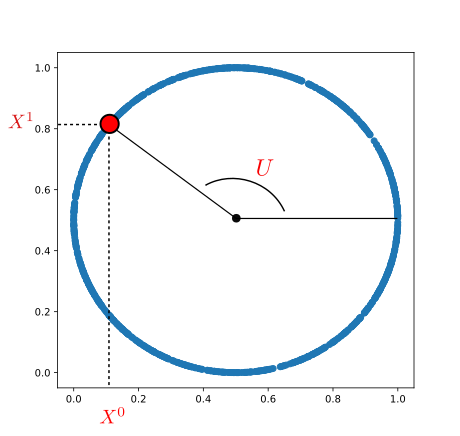
\includegraphics[width=0.6\textwidth]{cercle.pdf}
\end{minipage}
\begin{minipage}{0.5\textwidth}
\centering
\includegraphics[width=0.6\textwidth]{cercle_2.pdf}
\end{minipage}
\label{fig:U}
\caption{Exemples de paramétrisations du cercle. La paramétrisation qui traduit le plus facilement le modèle est naturellement celle dans laquelle $U$ est à valeurs réelles. Le modèle auxquelles appartiennent les modalités $X^0$ et $X^1$ est donc représenté par la variable cachée $U$.}
\end{figure}

\section{Présentation de l'expérience}

Nous étudierons dans ce chapitre l'organisation d'une architecture de deux cartes. L'architecture est illustrée à droite en figure~\ref{fig:exp}: elle est composée de deux cartes en une dimension. Chaque carte prend une entrée externe. Il s'agit de $\inpx\m{1}=x$ et $\inpx\m{2}=y$, les coordonnées de points 2D sur un cercle. Ces deux modalités sont dépendantes: pour une valeur de $x$, seule deux valeurs sont possible pour $y$, et symétriquement. Les entrées sont représentées sur le schéma de gauche, figure~\ref{fig:exp}.
Ces entrées externes sont normalisées entre 0 et 1. Les deux cartes sont des lignes 1D de 500 noeuds. Les rayons de voisinage sont $h_e = 0.2$ et $h_c = 0.02$.
Chacune des deux cartes est également connectée à sa voisine, c'est à dire, la carte $M\m{1}$ prend en entrée contextuelle la position du BMU de $M\m{2}$, et inversement.
Les données relatives à cette expérience et le code permettant de faire les tracés sont fournies sur git.

\begin{figure}
\begin{minipage}{0.4\textwidth}
\centering
\includegraphics[width=0.8\textwidth]{2som_inp_noinformation}
\end{minipage}
\begin{minipage}{0.6\textwidth}
\includegraphics[width=\textwidth]{2som_archi}
\end{minipage}
\caption{Disposition des entrée, sous forme de cercle, à gauche, et architecture de deux cartes en une dimension étudiée et représentée dans ce chapitre.\label{fig:exp}}
\end{figure}
\section{Représentation des cartes de Kohonen}

\subsection{Représentation des éléments des cartes}

Le jeu de données d'entrée se décompose en jeu d'apprentissage et jeu de tests. Lors de la phase de test, seul le processus de recherche de la best matching unit est réalisé et les poids des cartes ne sont pas mis à jour. Les éléments des cartes peuvent donc, comme les entrées, être considérés comme des variables aléatoires et une itération de test comme une réalisation de celles-ci. La phase de test peut être réalisée après n'importe quelle itération de l'algorithme d'apprentissage. Le processus d'apprentissage et de tests est décrit en figure~\ref{fig:flowchart}.

Nous considérerons plusieurs éléments des cartes; qui nous intéressent particulièrement dans les représentations, en tant que variables aléatoires: 
\begin{itemize}
\item Les positions des BMUs $\bmu\m{0}, \cdots, \bmu\m{n}$ dans chaque carte
\item Les poids externes des BMUs $\w_e\m{0}(\bmu\m{0}), \cdots, \w_e\m{n}(\bmu\m{n})$
\end{itemize}
Mais tout autre élément d'une carte peut être vu de cette manière, telles que les activités.


Une phase de test est alors un ensemble de réalisations d'une variable aléatoire jointe : 
$$(\inpx\m{0}, \cdots, \inpx\m{n}, \bmu\m{0}, \cdots, \bmu\m{n}, \w_e\m{0}(\bmu\m{0}), \cdots, \w_e\m{n}(\bmu\m{n}))$$
Les composantes de cette variable jointe ne sont pas indépendantes. Les représentations et indicateurs présentés ensuite chercheront à détecter et comprendre au mieux leurs dépendances statistiques.

Le formalisme par variable aléatoires permet d'utiliser des outils et métriques issus de la théorie de l'information pour qualifier l'organisation des cartes au sein de l'architecture.

\begin{figure}
\centering
\includegraphics[width=0.85\textwidth]{tests_2maps.pdf}
\caption{Schéma descriptif des tests}
\label{fig:flowchart}
\end{figure}


\section{Représentations graphiques}

La représentation classique d'une carte, qui est de tracer les poids par rapport à la position des unités de la carte, permet de visualiser la continuité des poids de la carte. 
Si on veut représenter quelle unités seront effectivement BMU et lesquelles ne le seront jamais, on y ajoute le tracé, sur un ensemble de tests assez grand, des poids des BMU en fonction des BMUs. Ces points se superposent à la courbe de poids, mais certaines unités ne seront pas représentées: on les appelles \emph{unités mortes}. La position de la best matching unit $\bmu$ étant la réponse de la carte à une entrée, il s'agit d'un tracé d'un élément de la carte en fonction de la réponse de celle-ci. 
Cette façon de représenter les réponse d'une carte rappelle directement la façon de représenter les neurones en biologie pour réaliser des cartes du cortex. Dans ces représentations, la valeur d'entrée faisant réagir un neurone est tracé en fonction de sa position dans le cortex.

Le poids de la BMU n'est pas le seul élément qu'on peut tracer en fonction de la réponse $\bmu$. Nous présentons dans cette partie les choix de tracés que nous utiliserons dans cette thèse.

\subsection{Représentation des entrées par rapport au BMU}

\subsubsection{Méthode}
En première représentation, nous tracerons la valeur de l' entrée $\inpx\m{i}$ d'une carte par rapport à la position du BMU $\bmu\m{i}$. Cette représentation permet d'analyser la quantification des entrées par la carte. Ces tracés sont réalisables pour des cartes une et deux dimensions, et pour des entrées quelconques, que ce soient des réels ou des entrées de plus grandes dimension comme des images.
Pour mieux comprendre les relations entre entrées et plusieurs cartes, on tracera sur une même figure les entrées de toutes les cartes selon la position du BMU d'une des cartes. Afin de comparer le comportement d'une carte de CxSOM avec une carte de Kohonen classique, on réalise le même tracé d'entrées par rapport au BMU, sur une carte qui aura appris indépendamment les mêmes valeurs de $\inpx\m{1}$ que $M\m{1}$, sans avoir de connexions avec $M\m{2}$. Cette dernière carte a donc seulement une couche de poids externes, il s'agit d'une carte de Kohonen classique.

On s'attend à ce que les entrées externes soient proche de la courbe de poids externes. Cela indiquera que le poids externe $\w\ext\m{1}(\bmu\m{1})$ est une approximation de $\inpx\m{1}$ et qu'une carte réalise de la quantification vectorielle sur ses entrées externes, malgré les connexions à l'autre carte. On attend également que la présence de la connexion avec $M\m{2}$, par l'entrée contextuelle, influence l'organisation de $M\m{1}$; et, si possible, qu'un modèle de connexions d'entrée est appris.

Ce tracé est présenté en figure~\ref{fig:inputs}. On représente la valeur des entrées $\inpx\m{1} = x$, en orange, et $\inpx\m{2}=y$, en bleu, par rapport à la position du BMU dans la carte $M\m{1}$, $\bmu\m{1}$. Ce tracé sur l'architecture de deux cartes (c) est comparé à ce qu'on obtient si les valeurs de $x$ étaient présentés à une carte classique (b). Les poids externes sont représentés en bleu, les poids contextuels en orange. Deux échantillons du schéma des entrées (a) sont mis en valeur, en bleu et rouge. Ces deux points ont la même valeur pour $x$, mais deux valeurs différentes pour $y$. Ces échantillons sont reportés en couleur sur les deux tracés (b) et (c).
\subsubsection{Résultats}
Analysons d'abord la forme des poids contextuels de $M\m{1}$, que nous avions tracés en figure~\ref{fig:weights} sans les commenter. Les poids externes, en orange, présentent une disposition similaire à ceux observés dans la carte classique (b). Les poids contextuels, en bleu, présentent une forme de vagues, avec 7 valeurs de maximum allant de 0.5 à 1, et 6 minimum allant de 0.5 à 0.1. Ces maximum et minimum sont répartis en zones de taille équivalente sur la carte. 

Lorsqu'on s'intéresse au tracés des échantillons, on remarque d'abord que les positions dans la carte $M\m{1}$ se répartissent en zones étant BMUs et zones mortes, dans lesquelles aucune entrée n'a gagné. C'est une première différence avec la carte indépendante, pour laquelle toutes les positions gagneront pour des entrées. Les zones dans lesquelles il y a des BMUs correspondent aux extremum des poids contextuels et leurs alentours. C'est un phénomène inhabituel pour une carte de Kohonen. Les entrées $\inpx\m{1}$, dans la carte classique (b), correspondent à la courbe de poids externe: la valeur du poids du gagnant est toujours très proche de la valeur de l'entrée. Dans la carte $M\m{1}$, les entrées externes $\inpx\m{1}$ orange sont proches de la courbe de poids externes, mais avec plus d'erreur de quantification.
Les deux points rouge et bleu ayant la même valeur de $x$ ont un BMU différent dans la carte $M\m{1}$, alors que ces deux échantillons ont le même BMU dans la carte apprenant indépendamment sur les valeurs de $x$. Ainsi, la carte connectée au sein de CxSOM différencie les échantillons en fonction de non seulement leur entrée externe, mais aussi de l'entrée de l'autre carte de l'architecture. La plage de valeurs des $\inpx\m{1}$ gagnant dans un des zones recoupe les plages de valeurs gagnant dans les zones situées à gauche et à droite. Par exemple, la zone dans laquelle l'échantillon rouge gagne, autour de $\bmu\m{1} = 0.25$. La partie des entrées située en dessous de la courbe de poids externe recoupe les valeurs d'entrées gagnant dans la zone précédente; la partie située au dessous de la courbe de poids externe recoupe des valeurs gagnant dans la partie suivante. Pour une entrée externe, le choix de la zone de BMU dans laquelle elle gagnera dépend alors de l'entrée contextuelle. 

\subsubsection{Conclusion}

Dans la carte $M\m{1}$, une unité se spécialise donc par rapport aux deux entrées et non pas une seule comme dans la carte indépendante: les entrées externes et l'entrée contextuelles. C'est bien ce à quoi on s'attendait en ayant deux couches de poids. Ce qui est intéressant est que cette différenciation est réalisée par la répartition des unités en un nombre fini de zones distinctes. Dans chaque zone, les unités sont BMUs pour un segment de valeurs d'entrée externe et contextuelles. Au sein d'une zone, la répartition des entrées externe selon le BMUs est ordonnée, comme ce serait le cas dans une carte auto-organisatrice classique. Le comportement de la carte au sein d'une zone reste donc similaire à celui d'une carte classique.

Deux zones adjacentes correspondent par ailleurs à des segments de valeur d'entrée en partie superposés, et des segments de valeurs d'entrées contextuelles différentes. Il s'agit d'une deuxième échelle d'organisation, qui garde également l'aspect ordonné d'une carte classique. Ces zones sont créées par auto-organisation; aucun paramètre de la carte n'a été modifié pendant l'apprentissage pour former ces zones, et le nombre d'unités allouées par auto-organisation dans chaque zone est à peu près égal. La carte agit un peu comme une base de données structurée avec des indices primaires et des indices secondaires pour chaque neurone, l'indice primaire étant la zone de la carte, et l'indice secondaire la position dans cette zone.

\begin{figure}
\begin{minipage}{0.27\textwidth}
\includegraphics[width=\textwidth]{2som_inp.pdf}
\end{minipage}
\begin{minipage}{0.34\textwidth}
\includegraphics[width=\textwidth]{weights_2som_unco.pdf}
\end{minipage}
\begin{minipage}{0.38\textwidth}
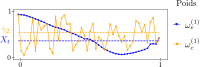
\includegraphics[width=\textwidth]{weights_2som.pdf}
\end{minipage}

\caption{Représentation des entrées $X$,$Y$ d'une architecture de deux cartes relativement au BMU de la carte $X$ après apprentissage. Ces tracés mettent en valeur l'organisation des cartes, différentes dans le cas ou les cartes apprennent indépendemment leurs entrées~(b) ou sont connectées~(c). Les entrées correspondantes sont en figure~(a). Les points bleu et rouge reportés sur les tracés correspondent au même échantillon de test.\label{fig:inputs}}
\end{figure}

\subsection{Représentation de U par rapport au BMU}

\subsubsection{Méthode}

Dans le cas d'une architecture de deux cartes, il était facile de tracer les deux entrées sur un même graphique. 
Lorsqu'on augmente la dimension, il est pertinent de dégager des nouvelles valeurs qui représentent le modèle en plus faible dimension: il s'agit ici de la variable $U$. 
Cette variable cachée est en fait une représentation du modèle en dimension plus faible. 
On peut tracer $U$ en fonction de la position $\bmu$ du BMU d'une carte pour représenter comment la position du BMU traduit la relation entre les entrées. Dans le cas de l'expérience à deux cartes, $U$ est en une dimension: il s'agit de l'angle correspondant à la position d'un point $x,y$ sur le cercle. 
On tracera donc $U$ en fonction de $\bmu\m{1}$ et $U$ en fonction de $\bmu\m{2}$. Nous avons observé sur les tracés en figure~\ref{fig:inputs} que chaque carte allouent leurs unités en fonction des deux entrées. En tracant $U$ en fonction de la position du BMU, on retrouvera d'abord les zones de la cartes. 

\subsubsection{Résultats}

Le tracé en figure~\ref{fig:piu} montre $U$ comme une fonction de la position du BMU dans chaque carte, contrairement au cas ou les cartes ne sont pas connectées. 
En effet, dans ce dernier cas, il y a plusieurs valeurs de $U$ pour un même $\bmu$, une valeur $x$ de $\inpx\m{1}$ correspondant à deux positions sur le cercle.
L'organisation en zones rend une position $\bmu$ codant pour une seule valeur de $U$, c'est à dire une seule position d'échantillon sur le cercle. $U$ est alors une fonction de $\bmu$, ce qui est représenté en pointillé sur la figure~\ref{fig:piu}. Donc, chaque carte $M\m{1}$ et $M\m{2}$ code pour toute l'architecture, par les deux couches de poids, et non plus seulement son entrée.

La forme générale du tracé de $U$ selon $\bmu\m{i}$ dans chaque carte est proche du tracé obtenu dans le cas des cartes indépendantes. Une carte de l'architecture se comporte donc comme une carte classique, dans laquelle les connexions contextuelles viennent moduler la réponse. La réponse d'une carte garde une continuité par rapport à $U$.
\begin{figure}
\centering
\includegraphics[width = 0.7\textwidth]{xu_yu_both.pdf}
\caption{Valeur de $U$ en fonction des valeurs du BMU $\bmu\m{i}$ dans chacune des cartes, pour des entrées prises sur le cercle. Sur la première ligne, nous tracons la réponse de chaque carte à son entrée dans le cas ou les cartes ne sont pas connectée. Sur la deuxième ligne, nous traçons la réponse de chaque carte lorsqu'elles ont appris de façon jointe au sein de CxSOM.
$U$ apparaît alors comme une fonction de la position du BMU $\bmu\m{i}$ dans chaque carte, contrairement au cas ou les cartes apprendraient indépendamment sur les mêmes entrées. Cette relation fonctionnelle est symbolisée par les pointillés sur les tracés du bas.}
\label{fig:piu}
\end{figure}

\subsubsection{Conclusion}
La représentation de $U$ selon la position du BMU d'une carte $\bmu\m{i}$ permet de représenter comment la carte $i$ a appris l'ensemble d'entrées $(\inpx\m{1},\inpx\m{2})$ et non seulement son entrée externe.

\subsection{Représentation de l'erreur de quantification dans une carte}

Afin de mesurer la qualité de la quantification vectorielle au sein d'une carte dans CxSOM, nous tracerons, pour un échantillon test, le poids externe du BMU $\w_e(\bmu\m{i})$ en fonction de l'entrée présentée $\inpx\m{i}$. 
Si une carte a appris bonne représentation correcte de ses entrées externes, la forme de ce tracé doit être proche de l'identité. 

En figure~\ref{fig:erreur}, nous avons tracé le poids du BMU de chaque carte en fonction de l'entrée qui lui a été présentée, dans l'expérience à deux cartes. Ces tracés s'approchent de l'identité: la quantification des entrées est correctement réalisée. On observe une erreur plus grande que dans le cas d'une carte isolée qui aurait le même nombre de neurones, c'est à dire 500 ici. Dans ce dernier cas, les 500 neurones permettent aux poids de se disposer densément entre 0 et 1..

\begin{figure}
    \centering
    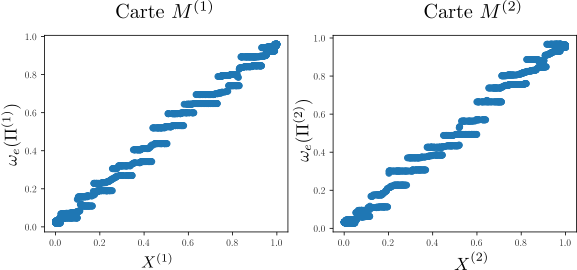
\includegraphics[width=0.7\textwidth]{w_x.pdf}
    \caption{Poids du BMU dans chaque carte en fonction de l'entrée présentée. On s'attend à des tracés proches de l'identité, montrant que le poids du BMU d'une carte est une bonne représentation de l'entrée. Sur ce graphique, on se rapproche effectivement de la fonction identité, cependant, une faible erreur est observée. On observe également un découpage des poids en bandes.\label{fig:erreur}}
\end{figure}

\draft{\subsection{Dépliement d'une carte en plusieurs dimensions}

\subsubsection{Méthode}
Nous avons vu qu'analyser le comportement d'une carte en fonction de toutes les entrées est un moyen de mieux comprendre la représentation interne qu'a une architecture sur le modèle d'entrée.
Nous proposons ici une façon originale de représenter les poids d'une carte de Kohonen dans l'espace de toutes les entrées. Cette représentation est faisable lorsque la dimension totale des entrées est de deux ou trois. Nous utiliserons donc cette représentation seulement sur les données géométriques, afin de mieux comprendre l'organisation des cartes.

Cette représentation est crée à partir des échantillons de test. Il s'agit de tracer les poids externes des BMUs dans l'espace de toutes les entrées: $(\w_e(\bmu\m{1}),\cdots,\w_e(\bmu\m{k}))$ dans l'espace en $k$ dimensions correspondant - $k$ correspondant ici à 2 ou 3 dimensions. Les échantillons sont ensuites reliés suivant l'ordre des positions dans \emph{une des cartes}. On obtient ainsi le \emph{dépliement} d'une carte de l'architecture dans l'espace multimodal à plusieurs dimensions. 

\subsubsection{Résultats}

Un exemple de carte ainsi dépliée est présenté en figure~\ref{fig:distortion}.

\begin{figure}
\begin{minipage}{0.5\textwidth}
\centering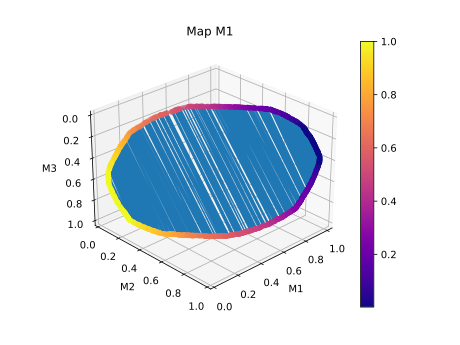
\includegraphics[width=0.8\textwidth]{unco3som}
\end{minipage}
\begin{minipage}{0.5\textwidth}
\centering\includegraphics[width=0.8\textwidth]{disto_Mx}
\end{minipage}
\caption{Représentation des poids finaux de trois cartes prenant en entrée les coordonnées des points d'un cercle: $x = \inpx\m{1}$,$y = \inpx\m{2}$ et $z=\inpx\m{3}$, reliés selon les positions de la carte $X$. A gauche, les cartes de l'architecture ont appris séparément sur les données. A droite, disposition lorsque les cartes ont été connectées au sein d'une architecture. Un échantillon de 1000 points a été utilisé pour les tracés.}
\label{fig:distortion}
\end{figure}

Ces figures sont équivalentes à tracer une carte dans l'espace de ses entrées: les poids des BMUs de l'échantillon sont les prototypes des cartes; seuls les poids des unités mortes ne sont pas représentés.
Cette représentation est limitée par la dimension des entrées, mais elle peut-être étendue: en plus grande dimension, il est possible de tracer le dépliement de la carte selon un sous-espace choisi de chacune des modalités, ou après réduction de dimension.
Par ailleurs, l'étude du comportement de cartes sur des données 3D s'inscrit dans la démarche de construction d'un modèle que nous suivons dans cette thèse. Leur visualisation est alors un élément clé dans la compréhension des comportements possibles de l'architecture. A partir de cette visualisation, on peut envisager de construire des indicateurs permettant l'analyse de l'architecture en dimension supérieure. 

Le second avantage de ces tracés est qu'il est possible de représenter graphiquement une carte qui ne prend pas d'entrée externe, ou de représenter une carte dans l'espace des poids d'autres cartes.
}

\section{Information mutuelle comme indicateur statistique}

L'étude de tout processus physique s'effectue par un ensemble signaux issus de capteurs. La théorie de l'information de Shannon \cite{Shannon1948AMT} apporte un modèle mathématique qui abstrait ces signaux et permet de les manipuler, les encoder, les décoder et quantifier l'apport ou perte d'information entre eux, en les utilisant en tant que distributions de probabilités.
Ce modèle mathématique puissant permet de s'abstraire de la nature des signaux pour s'intéresser à leurs relations. Comme son nom l'indique, la théorie de l'information s'appuie sur la notion fondamentale d'information portée par un symbole. Ensuite, cette information se décline en quantités qu'on calcule en fonction de ce qu'on veut mesurer: l'entropie d'une variable, comme l'information apportée par l'observation de la variable seule; l'entropie conditionnelle entre deux variables,l'information mutuelle entre deux variables ou un plus grand nombre. Ces mesures définissent une dépendance statistique générale, et ne dépendent pas du type de modèle ou de relation.

Nous investiguerons dans cette partie comment quantifier l'apprentissage de l'architecture de cartes par des outils d'information. Bien que cette théorie soit un outil mathématique puissant, il s'agit d'un modèle s'appuyant sur les probabilités. L'estimation à partir de données est donc un élément clé et parfois limitant lorsqu'on cherche à utiliser des valeurs telles que l'entropie pour quantifier l'information au sein d'un système. Nous définirons donc dans cette partie des quantités à mesurer dans l'architecture de cartes, et chercherons à l'estimer.

\subsection{Information mutuelle et entropie}

Les notions d'\emph{entropie} et les valeurs qui en sont dérivées, telle que l'\emph{information mutuelle} entre des distributions, sont des notions fondamentales de la théorie de l'information de Shannon. Ces quantités donnent des informations concernant la distribution d'une variable aléatoire.
Les formules indiquées dans ce paragraphe concernent des variables aléatoire discrètes. 
L'entropie de Shannon d'une variable aléatoire $X$ à valeurs discrètes dans un ensemble $E_X$, de distribution $p(X)$, est notée $H(X)$ et définie par la formule : 
\begin{equation}
H(X) = - \sum_{x \in E_X}{p(x)\textrm{log}(p(x))}
\end{equation}

Elle se mesure en $bit/symbole$ lorsque le logarithme est en base 2, ce qui est généralement utilisé. 
L'entropie est une mesure de la quantité d'incertitude, ou de surprise, sur la valeur de la variable aléatoire $X$. Si la la distribution de probabilité de $X$ est concentrée autour d'un point, l'entropie est faible : lors d'une réalisation de $X$, l'observateur est \emph{plutôt certain} du résultat. En revanche, l'entropie est maximale lorsque lorsque $X$ suit une distribution de probabilité uniforme.
L'entropie s'interpète également comme la quantité moyenne d'information à fournir, en bits, pour coder la valeur que prend la variable $X$.
De la même manière, on peut définir l'entropie conjointe de deux variables, qui est l'entropie de leur distribution jointe, et l'entropie conditionnelle, qui est l'entropie de leurs distributions conditionnelles.

Outre les entropies jointes et conditionnelles, les relations statistques entre deux variables aléatoires $X,Y \in E_X,E_Y$ peuvent être mesurées par \emph{l'information mutuelle}. Elle se définit formellement par : 
\begin{equation}
 I(X,Y) = \sum_{x,y \in E_X,E_Y}{p(x,y)\textrm{log}(\frac{p(x,y)}{p(x)p(y)})}
\end{equation}
Cette valeur mesure la quantité d'information moyenne apportée par une réalisation de $X$ sur la réalisation de $Y$.

L'information mutuelle possède les propriété suivantes:
\begin{enumerate}
\item $I(X,Y) = 0 \Leftrightarrow \textrm{X et Y sont indépendantes}$. L'information mutuelle peut être vue une mesure de la distance entre la distribution jointe de $(X,Y)$, $p(X,Y)$ et la distribution dans laquelle les deux variables sont indépendantes, $p(X)p(Y)$.
\item Elle s'exprime à partir de l'entropie : $I(X,Y) = H(X) + H(Y) - H(X,Y) = H(X) - H(X|Y) = H(Y) - H(Y|X)$
\item Elle est symétrique : $I(X,Y) = I(Y,X)$
\item Pour toute fonction $f$, $I(X,Y) \geq I(X,f(Y))$. L'égalité est atteinte si et seulement si $f$ est \emph{bijective}.
\end{enumerate}


\subsection{Indicateur: Information mutuelle}

Lors de l'analyse de CxSOM, on s'interroge sur l'information que portent les positions des BMUs $\bmu$ d'une carte sur le modèle d'entrées. Les éléments de la carte ont été définis en terme de variables aléatoire; on peut donc utiliser l'information mutuelle comme une représentation de l'information portée par le BMU d'une carte sur le modèle. Le modèle est représenté par la variable $(X,Y,Z)$, mais aussi par $U$. $I(\bmu, U)$ est alors l'information moyenne que le BMU d'une carte porte sur $U$, donc sur le modèle, et $U$ sur le BMU. On souhaite cependant avoir un indicateur normalisé, qui permettrait, sur une échelle de 0 à 1, de quantifier à quel point un BMU porte de l'information sur $U$. On va donc normaliser l'information mutuelle $I(\bmu,U)$ par la valeur maximale qu'elle peut prendre dans notre carte.


Cette valeur maximale atteinte par $I(\bmu,U)$ est $H(U)$, atteinte lorsque $U$ est fonction de $\bmu$.
En effet, par construction, $\bmu$ est une fonction de $U$ dans une carte de Kohonen: l'algorithme est déterministe et une sortie est définie pour toute valeur de $U$. C'est à dire, $I(U,\bmu) = I (U, f(U))$.
Par propriété de l'information mutuelle, pour toute fonction $f$ et variables $X,Y$, $I(X,f(Y)) \leq I(X,Y) $. 
Donc, $I(U,\bmu) \leq I(U,U) = H(U)$
Cette valeur est atteinte si et seulement si $U$ et $\bmu$ sont en bijection, autrement dit, si et seulement si $U$ est aussi une fonction de $\bmu$.


Nous définissons donc un indicateur de la relation entre $U$ et un BMU comme:
\begin{equation}
I_x(U|\bmu) = \frac{I(\bmu,U)}{H(U)}
\end{equation}
Ce coefficient n'est pas symétrique, et mesure donc l'information portée par le premier terme sur le second, relativement à la valeur maximale qu'elle peut prendre. Dans le cas des cartes CxSOM, $I_x \in [0,1]$. Cette valeur rappelle le \emph{coefficient d'incertitude} entre $U$ et $\Pi$, ou $U$ de Theil \cite{Theil1961EconomicFA}.

%TODO : développer ce point : information portée par plus de variables !
%TODO : calculer et comparer les valeurs pour le cas du cercle.

Ce coefficient peut être élargi à plus de variables: on peut calculer $I_x(U | (\bmu\m{1},\bmu\m{2},\bmu\m{3}))$ pour 3 cartes, en considérant la variable jointe $(\bmu\m{1},\bmu\m{2},\bmu\m{3})$.
Plus largement, pour prouver que l'archictecture a appris un modèle, on souhaite que $I_x(U|\bmu\m{1},\cdots,\bmu\m{k})$ soit le plus proche possible de 1.

\comment{Qu'est ce que l'information portée par plusieurs variables représente dans le cas du cercle !}

\subsection{Evolution de l'information entre deux cartes}

\subsubsection{Estimation}
L'information mutuelle et l'entropie sont des grandeurs probabilistes. Elles sont définies à partir de la distribution des variables aléatoire. Lorsque qu'on ne connait pas les distributions, il est nécessaire d'estimer ces valeurs autrement. 
Nous estimons la distribution des variables $X$,$Y$ et leur distribution jointe $Z = (X,Y)$ en discrétisant l'espace par la méthode des \emph{histogrammes}, représenté en figure~\ref{fig:binning}. Les variables X et Y sont donc discrétisées en \emph{boîtes} de centres $x_k$ et $y_k$. La distribution de X est alors estimée par: 
$$P(X = x_i) = \frac{n_{xi}}{N} $$, où $n_{xi}$ est le nombre d'échantillons de X tombant dans la boîte de valeur $x_i$ et $N$ le nombre de points. Le même procédé est réalisé pour $Y$ et $Z = (X,Y)$. La précision de l'estimation peut être améliorée en choisissant des tailles de boîtes variables; nous utilisons ici la méthode simple avec des boites de taille fixe.
L'information mutuelle et l'entropie sont ensuite estimées à partir de ces distributions discrètes, par leur formules:
\begin{equation}
    I_x(X,Y) = \sum_{i = 0}^{n_x} \sum_{j=0}^{n_y} {P(x_i,y_j)\textrm{log}\left(\frac{P(x_i,y_j)}{P(x_i)P(y_j)}\right)}
   \end{equation}

\begin{figure}
\centering
\includegraphics[width=0.45\textwidth]{boxes}
\caption{Méthode par histogrammes pour estimer les distributions des variables $X$ et $Y$. Les distributions sont estimées à partir de $n_{xj}$, $n_{yi}$ et $n_{zij}$, puis les valeurs de l'entropie $H$ et l'information mutuelle $I$ calculées.}
\label{fig:binning} 

\end{figure}

%\begin{figure}
%\centering
%\includegraphics[width=\textwidth]{mutual_info_evol.pdf}
%\caption{Evolution de l'indicateur relatif à l'information mutuelle entre $\Pi$ et $U$ dans chaque carte au cours de l'apprentissage. Cet indicateur est comparé à celui calculé dans le cas ou les cartes apprennent séparément.}
%\label{fig:im} 
%\end{figure}

\subsubsection{Information mutuelle sur deux cartes}
Analysons à présent comment l'information mutuelle évolue au cours de l'apprentissage dans un système de deux cartes apprenant sur le cercle en deux dimensions.

Pour cette expérience, une phase de test sur 5000 entrées test est réalisée toutes les 10 itérations, puis toutes les 200 itérations à partir de l'itération 200. Chaque phase de test donne alors un ensemble d'entrées $\inpx\m{1}, \inpx\m{2}, U$ et un ensemble de réponses des cartes $\bmu\m{1}, \bmu\m{2}$. On peur alors estimer $I_x(U|\bmu\m{1})$ et $I_x(U|\bmu\m{2})$ sur chaque itération considérée, ce qui nous donne la courbe de l'évolution de l'indicateur au long de l'apprentissage. 
Ces calculs sont réalisés sur 100 apprentissages complets, prenant des entrées d'apprentissage aléatoires sur le même cercle. Les cartes sont initialisées à des poids aléatoires au début de chaque apprentissage. 
Les tracés présentés en figure~\ref{fig:MI_evol}, sont la moyenne, à chaque pas de temps, de l'information mutuelle de chaque expérience au pas de temps $t$. On représente donc l'évolution de l'information mutuelle en moyenne. 

Nous comparons les valeurs obtenues pour une carte de CxSOM à celles d'une carte apprenant sur les mêmes entrées $\inpx\m{1}$ ou $\inpx\m{2}$, mais sans connexions entre elles. On s'attend à ce que l'information soit plus élevée pour la carte au sein de CxSOM que la carte seule, ce qui montrerait que la carte porte aussi de l'information sur l'autre entrée. On s'attend à ce que cette valeur atteigne 1, ce qui montrerait qu'une seule carte porte de l'information sur tout le modèle: $U$ est une fonction de $\bmu$ dans chaque carte.

L'estimation est réalisée par la méthode des histogrammes. On choisit une taille de boite de 50 pour $U$ et 500 pour $\bmu\m{i}$; de cette façon, les points correspondant à des $U$ très proches seront comptés ensemble pour l'estimation de l'information.

L'observation du tracé montre qu'en effet, les informations mutuelles $I_x(U|\bmu\m{1})$ et $I_x(U|\bmu\m{2})$ sont toutes deux plus élevées à chaque moment de l'apprentissage que dans le cas ou les cartes sont séparées. C'est également vrai au tout début de l'apprentissage: en effet, les BMUs étant calculés selon les poids contextuels et les poids externes

Cette valeurs augment rapidement et se stabilisent autour de 0.8. Cette stabilisation correspond à la stabilisation des poids de l'architecture.

\begin{figure}
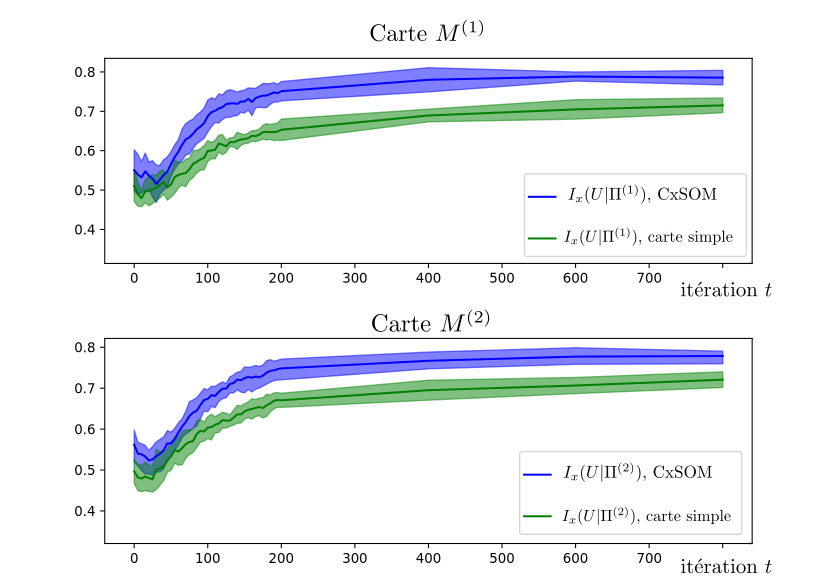
\includegraphics[width=\textwidth]{evolution_MI_binning}
\caption{Evolution du coefficient d'incertitude dans chaque carte au long de l'apprentissage. La courbe bleue correspond à $I_x(U|\bmu)$ dans l'architecture de cartes $M\m{1}$ et $M\m{2}$. On compare cette évolution à l'évolution de l'information d'une seule carte apprenant sur les mêmes entrées $X$ ou $Y$, sans être connectée.}
\label{fig:MI_evol}
\end{figure}

\subsection{Discussion}
\subsubsection{Influence de l'estimation}
Lorsque la dimension augmente, le nombre d'échantillon disponibles doit augmenter exponentiellement avec la dimension des variables pour éviter le phénomène de "boîtes vides": à cause de la dispersion des données, de nombreuses boîte $(x_j,y_i)$ ne contiendront pas de points alors qu'elles auraient du en contenir selon leur distribution; l'estimation de la probabilité en ce point sera donc nulle, et l'estimation faussée. 

Nous avons donc envisagé d'autres estimateurs moins biaisés en grand dimension. Détaillons par exemple l'estimateur par KNN (K-nearest neighbors) de Kraskov \cite{2004kraskov}. 
Cet estimateur ne passe pas par l'estimation de la densité de probabilité, contrairement aux histogrammes, mais estime directement l'information mutuelle. C'est l'estimation de la densité de probabilité qui posai justement problème en grande dimension.
Le découpage de l'espace se fait en recherchant, pour un couple $(X,Y)$ les k plus proches voisins. Une information mutuelle locale est calculée dans cette zone de l'espace, suivant une formule permettant d'approximer les différences de logarithme par la fonction digamma $\psi$ : 
$$i_j(X,Y) = \psi(k) - \psi(n_{x_j} + 1) - \psi(n_{y_j} +1) + \psi(N)$$
Cette information mutuelle locale est ensuite moyennée sur l'ensemble des points: 
$$\hat{I}(X,Y) = \psi(k) - \langle\psi(n_{x_j} + 1) + \psi(n_{y_j} +1)\rangle + \psi(N)$$
Pour estimer $I_x(X|Y)$, on estimera $I(X,Y)$ et $H(Y)$ avec les mêmes paramètres, en notant que $H(Y) = I(Y,Y)$.

Comparons les deux méthodes d'estimation de l'information mutuelle proposées dans ce chapitre: l'estimation par histogrammes, et l'estimation par KNN de Kraskov.
En figure~\ref{fig:MI_evol_total}, nous tracons l'évolution de l'information mutuelle moyenne, cette fois estimée par la méthode de Kraskov. Sur le même schéma, nous tracons également l'évolution de l'information mutuelle obtenue par la méthode des histogrammes. 

Sur les tracés, l'indicateur calculé avec la méthode de Kraskov converge vers une même valeur à la fin de l'apprentissage pour la carte simple que pour la carte au sein d'une architecture CxSOM (tracés rouges et noirs). Ce résultat est étonnant: cela signifie donc que la carte au sein de CxSOM n'a pas plus d'information sur le modèle que la carte isolée, lorsque cette information est estimée avec la méthode de Kraskov. Ce résultat va également à l'encontre de ce qu'on observe sur l'évolution de l'information mutuelle calculée par les histogrammes, dans laquelle une différence franche est observée entre la carte isolée et la carte au sein de l'architecture.

Proposons une explication.
La méthode des noyaux de Kraskov est plus "granulaire" que la méthode des histogrammes au niveau de l'estimation, c'est à dire que les données sont considérées \emph{points par point}. L'avantage est que l'évaluation de la relation fonctionnelle entre $U$ et $\bmu\m{i}$ est plus précise qu'avec les histogrammes: s'il y a deux valeurs de $U$ pour un même $\bmu\m{i}$, l'information diminue. Par contre, la contribution de ces deux valeurs sera la même dans le calcul de l'information mutuelle, qu'elles soient proches ou éloignées: la distance entre donnée n'intervient pas dans le calcul. Cette différence de contribution est illustrée en figure~\ref{fig:exemple-limite}. On calcule l'information mutuelle $I_x$ dans les deux cas de distribution proposées, à l'aide de l'estimateur granulaire de Kraskov. Dans le cas ou la relation est proche d'une relation fonctionnelle, mais est très bruitée, l'information $I_x(Y|X)$ est plus faible que dans le cas ou cette relation n'est pas fonctionnelle, mais sans bruit parasite.

On observe que l'information $I_x(U|\bmu)$ tend vers une même valeur dans CxSOM et dans une carte isolée quand on la calcule avec l'estimateur granulaire. Cela signifie, qu'on a la même quantité d'information sur $U$ avec le BMU, dans la carte isolée que dans CxSOM. Simplement, cette information n'est pas répartie de la même façon. 
Dans une carte isolée, le niveau de quantification vectorielle qu'on effectue sur $X$ est très précis: lorsqu'on présente une entrée $X$ à la carte, le poids du BMU est très proche de cette valeur $X$ Dans CxSOM, on perd ce niveau de quantification, ce qu'on a observé en figure~\ref{fig:erreur}. Le fait que l'indicateur, lorsqu'il est estimé avec une méthode très granulaire, prend la même valeur dans les deux expériences traduit alors qu'on a perdu de l'information sur l'entrée $X$ par rapport à la carte isolée, avec la perte de précision, mais qu'on a gagné de l'information sur l'autre entrée $Y$. Le fait que les deux évolutions de $I_x$, pour chaque expérience, convergent vers la même valeur montre qu'on est dans une situation de compromis: on gagne de l'information sur le modèle au détriment de l'information sur l'entrée externe.

C'est donc le fait de discrétiser grossièrement la distribution de $U$ qui permet de mesurer le gain d'information sur le modèle complet, sans prendre en compte le fait que la précision sur l'entrée externe est affaiblie. L'indicateur $I_x$ reste un indicateur fiable, mais il doit être utilisé en prenant en compte cet aspect.

%ela a peu de sens dans le cas de notre application: on souhaite mesurer que $U$ est proche d'une fonction de $\bmu$, mais du bruit est toléré. L'estimation par histogrammes permet de ne pas prendre en compte ce bruit; ce n'est pas possible avec la méthode de Kraskov. 



\begin{figure}
    \centering
    \includegraphics[width=0.35\textwidth]{kraskov.pdf}
    \caption{Découpage en KNN de Kraskov pour estimer l'entropie et l'information mutuelle des variables $X$ et $Y$. Les plus proches voisins du point rouge sont trouvés, en vert, et le processus est répété sur tous les points. Les valeurs de $n_x$ et $n_y$ permettent d'estimer directement l'entropie.}
    \label{fig:kraskov}
\end{figure}

\begin{figure}
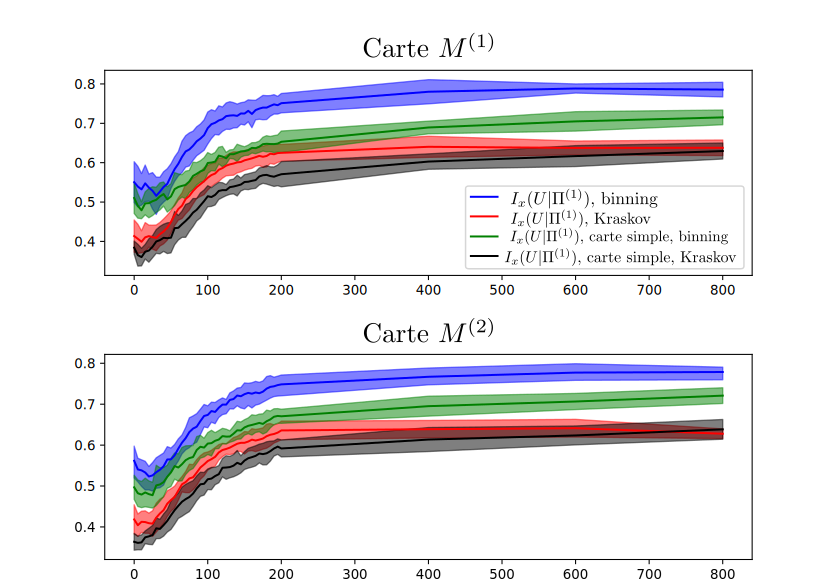
\includegraphics[width=\textwidth]{evolution_MI}
\caption{Evolution du coefficient d'incertitude dans chaque carte au long de l'apprentissage, en comparant l'estimation par histogrammes et l'estimation par la méthode de Kraskov.}
\label{fig:MI_evol_total}
\end{figure}

\begin{figure}
    \centering
    \includegraphics[width=\textwidth]{comparaison_binning_kraskov.pdf}
    \caption{Comparaison du calcul de l'indicateur $I_x$ sur deux distributions. A gauche, la relation entre $Y$ et $X$ se rapproche d'une fonction, mais bruitée. A droite, la relation n'est pas fonctionnelle, mais de telle sorte qu'une valeur de $X$ correspond au maximum à deux valeurs de $Y$. Lorsqu'on calcule l'indicateur avec la méthode très granulaire de Kraskov, cet indicateur est plus élevé dans le cas de droite que de gauche: en effet, le calcul ne prend pas en compte si les points sont condensés ou éloignés. Pour que l'indicateur nous informe correctement sur l'aspect fonctionnel de la relation entre $X$ et $Y$, il faut enlever manuellement le bruit. Avec la méthode par histogrammes, on prend une taille de boîte de $0.1$ selon $Y$. Dans ce cas, l'indicateur est bien plus élevé à gauche, ou $Y$ se rapproche d'une fonction de $X$, que à droite.}
    \label{fig:exemple-limite}
    \end{figure}

\subsubsection{Perspectives}

L'indicateur que nous proposons, $I_x(Y|X) = \frac{I(X,Y)}{H(Y)}$ traduit bien le fait que les cartes ont appris une relation entre les entrées. Son estimation doit passer par une discrétisation avec des intervalles larges pour $U$, afin de ne pas prendre en compte la perte d'information sur l'entrée externe $X$.
Les données doivent égalemement être débruitées avant l'estimation.
L'information mutuelle et l'entropie étant des quantités fondamentales en théorie de l'information, il existe de nombreuses méthodes d'estimations de ces valeurs malgré la difficulté qu'elle pose, voir~\cite{Doquire2012ACO} pour une revue de différentes méthodes. Ainsi, l'utilisation du coefficient d'incertitude comme indicateur reste robuste pour des données de plus grande dimension ou pour plus de cartes, en utilisant des méthode d'estimations plus élaborées. Cependant, cette estimation devra être retravaillée en plus grande dimension. 

\draft{
Une solution serait par exemple de chercher à séparer les sources d'information: l'information apportée par $X$ sur $U$ de l'information apportée par $\bmu$ sur $U$. On pourrait alors mesurer un gain d'information. Par exemple, en~\cite{williams_nonnegative_2010}, les auteurs décomposent l'information à plusieurs variables en \emph{redondance} et \emph{synergie}. 
}


% \draft{
% \subsection{Autre indicateur: le ratio de core}

% L'indicateur correlation ration permet de mesurer la distance d'une distribution à la fonction qui la fitte. Cela correspond bien à ce qu'on cherche dans CxSOM, mais estimation complexe aussi en grand dimension. 
% }

\section{Conclusion}
\begin{itemize}
\item La représentation par échantillonnage et variable aléatoire permet de mieux comprendre les mécanismes des cartes, ceux ci ne reposant plus directement sur les courbes de poids
\item Ces tracés montrent qu'une architecture de deux cartes s'organise comme une carte simple, mais modulée par l'entrée contextuelle: les poids externes se déplient comme une carte simple, mais les poids contextuels amènent des zones dans la carte. Ces zones séparent les BMUs en fonction de à la fois les entrées externes (organisation générale), et des entrées contextuelles (localement). Observation d'un nombre réduit de zones. 
\item Perte de précision au niveau de la quantification des poids externes, mais apprentissage d'un modèle. Nécessité de faire un compromis, réalisé de façon auto-organisée. Chaque carte a alors appris le modèle en entier et non seulement son entrée.
\item Utilisation d'un indicateur basé sur l'info mutuelle pour évaluer comment une carte apprend le modèle. Indicateur pouvant être utile en grande dimension ; mais l'estimation peut poser problème à ce moment.
\end{itemize}


\comment{Correlation ration : mesure de dépendance fonctionnelle
Débruitage de l'IM : répétition de l'expérience et moyenne ?}
\draft{Le ration de corrélation traduit mieux que le coefficient d'incertitude la dépendance fonctionnelle entre le modèle et le BMU. Cependant, à l'inverse de l'information mutuelle, une relation non fonctionnelle mais précise (telle que l'exemple du cercle de la figure~\ref{fig:exemple-limite}) entre les variables aura un score très faible. Ce n'est pas non plus voulu. 

Il semble que l'information mutuelle reste le moyen le plus prometteur et le plus général de mesurer la relation entre les éléments des cartes. Dans le cas une dimension, on observe qu'on veut tendre vers U fonction du BMU; on connait mal le comportement recherché en dimension plus grande (cartes 2D, entrées de grande dimension). L'information mutuelle laisse donc l'opportunité à plus d'états d'organisation des cartes de l'architecture d'avoir un bon score. La meilleure perspective serait donc de pouvoir calculer le coefficient d'incertitude sur des échantillons provenant de données non bruitées, ou de pouvoir séparer le bruit des données lors du calcul du coefficient.
Dans cette optique, l'estimateur par histogrammes permet de réduire l'effet du bruit, en choisissant correctement les tailles de boîtes. L'utilisation histo versus Kraskov reste donc à discuter.
Dans le cas ou le modèle d'entrée est connu, calculer les réponses des cartes sur des jeux de données non bruitées générées artificiellement, après apprentissage sur un jeu de données réelles et bruitée, est une solution. Si le modèle n'est pas connu, des méthodes statistique de réduction de bruit peuvent être imaginées.} 

\draft{
\section{Prédiction d'entrée}

Au sein d'une architecture de cartes, il est possible de ne pas présenter à une ou plusieurs cartes de l'architecture leur entrée externe $\inpx\m{i}$. Dans ce cas, une best matching unit peut quand même être calculée par leurs entrées contextuelles. Le poids de cette best matching unit peut alors être vu comme une prédiction de l'entrée manquante. Cette capacité de prédiction peut être à la fois vue comme une application possible de l'architecture, mais aussi comme une façon de représenter \emph{ce que les autre cartes connaissent d'une autre}. Tracer les prédictions d'une carte est donc un indicateur de la façon dont une architecture a appris des relations. 


\comment{
2 parties dans estimation/perspectives : 
d'une part, questionnement sur l'estimation des données bruitées par exemple - pas besoin de proposer des solutions si elles ne sont pas testées ? 
Et parler de l'estimation en grande dimension : ce n'est pas forcément le pb ici. Donc pas la peine...
}
}
